
\documentclass[twoside]{article}
\usepackage{amsmath}
\usepackage[english]{babel}

\usepackage[utf8]{inputenc}
\usepackage{geometry}
\usepackage[colorlinks=true, allcolors=blue]{hyperref}
\geometry{
  a4paper,
  total={170mm,257mm},
  left=20mm,
  top=20mm,
}
\usepackage{graphicx}
\DeclareGraphicsExtensions{.pdf,.png,.jpg}
\usepackage{float}
\usepackage{titling}
\usepackage{amsfonts}

% Use the package to disaply c++ code 
\usepackage{listings}
\usepackage{tikz}
\usepackage{xcolor}
\usepackage{wrapfig}
\usepackage{svg}
\usepackage{svg-extract}
\svgsetup{clean=true}

\lstloadlanguages{[Visual]C++, [ISO]C++}

\definecolor{codegreen}{rgb}{0,0.6,0}
\definecolor{codegray}{rgb}{0.5,0.5,0.5}
\definecolor{codepurple}{rgb}{0.58,0,0.82}
\definecolor{backcolour}{rgb}{0.98,0.98,0.98}
\definecolor{lightgreen}{rgb}{0.4,1,0.4}
\definecolor{lawngreen}{rgb}{0.48,0.99,0}
\definecolor{darkgrey}{rgb}{0.35,0.35,0.35}

\lstdefinestyle{mystyle}{
  language={[Visual]C++},
  % backgroundcolor=\color{backcolour},   
  commentstyle=\color{darkgrey},
  numberstyle=\tiny\color{codegray},
  stringstyle=\color{brown},
  basicstyle=\ttfamily\footnotesize,
  breakatwhitespace=false,         
  breaklines=true,                 
  captionpos=b,                    
  keepspaces=true,                 
  numbers=left,                    
  numbersep=5pt,                  
  showspaces=false,                
  showstringspaces=false,
  showtabs=true,                  
  tabsize=2,
  morekeywords={T, once, Neuron, NeuronNetwork, NeuronLayer},
  morekeywords=[2]{iostream, pow, emplace_back, static_cast, size, vector, array, push_back, insert, begin, end, reserve, 
  resize, capacity, cout, endl, generate, random_device, mt19937, uniform_real_distribution, empty, clear, size_t,
  atomic, thread, hardware_concurrency, ref, fetch_add, fetch_sub, joinable, fetch_sub, fetch_add, join, load,
  static, operator, front, back, max_element, min_element, Map, VectorXf, data, dot},
  morekeywords=[3]{malloc, free},
  keywordstyle=[3]\color{lawngreen},
  keywordstyle=[2]\color{red},
  keywordstyle=\color{blue}
}

\lstset{style=mystyle}

\title{Performance analysis neural network}
\author{Stan Merlijn}
\date{februari 2025}
 
\usepackage[headings]{fancyhdr}
% \pagestyle{headings}
\fancypagestyle{plain}{%  the preset of fancyhdr 
    \fancyhf{} % clear all header and footer fields
    % \fancyfoot[R]{\includegraphics[width=2cm]{KULEUVEN_GENT_RGB_LOGO.png}}
    % \fancyhead[L]{Performance analysis neural network}\
    \fancyhead[LE,RO]{\textsl{\rightmark}}
    \fancyhead[LO,RE]{\textsl{\leftmark}}
    \fancyhead[R]{Machine learning 2024\_TAAI-V2ML-19\_3\_V}
    \fancyfoot[L]{\thedate}
    \fancyfoot[R]{\thepage}
    \renewcommand{\headrulewidth}{0.4pt}
    \renewcommand{\footrulewidth}{2pt}
}

\makeatletter
\def\@maketitle{%
  \newpage
  \null
  \vskip 1em%
  \begin{center}%
  \let \footnote \thanks
    {\LARGE \@title \par}%
    \vskip 1em%
    {\large \@date}%
  \end{center}%
  \par
  \vskip 1em}
\makeatother

\usepackage{lipsum}
% \usepackage{cmbright}
\begin{document}

\maketitle

\noindent\begin{tabular}{@{}ll}
  Student                & \theauthor                                                                  \\
  Email                  & stan.merlijn@student.hu.nl                                                  \\
  Student number         & 1863967                                                                     \\
  % link github(origineel) & \url{} \\
  Link github(classroom) & \url{https://github.com/StanMerlijn/ML-sigmoid-neuron/tree/backpropagation} \\
  Testing framework      & Catch2\cite{catchorg-no-date}                                               \\
\end{tabular}

\section{Abstract}
In this essay, we discuss the performance improvements discovered during the development of a neural network.
This essay summarizes the insights gained throughout the process. Although this essay does not contribute to the overall grading,
it serves as a valuable reflection on the lessons learned during the assignment.


\tableofcontents

\pagestyle{plain}
\newpage

\section{Performance improvements}
\subsection{Baseline Perforamance}
Initially, the focus was on correctness rather than performance.
While the implementation was accurate, it was inefficient. For example,
training an XOR gate with 10,000 epochs using one hidden layer with 2 neurons and an output layer with a single neuron took approximately 190 ms.
Remarkably, this is slower than the native Python implementation (despite Python’s generally slower performance),
which clearly indicated that our C++ implementation needed optimization. The first and simplest improvement was to compile in release mode.
Since the project is built with \href{https://cmake.org/}{CMake} and the default build type is set to debug,
switching to release mode significantly reduced the training time to roughly 25 ms.
Further optimizations are discussed in the following chapters.

\subsection{Returning Vectors by reference}
Looking at the code, it was clear that the vectors were returned by value. This means that the vectors were copied every time they were returned.
Meaning that for every copy new allocations were made. To test the amount of allocations made, the \texttt{new} operator was overloaded.
\begin{lstlisting}
  static int s_Allocations = 0;

  void* operator new(size_t size) {
      s_Allocations++;
      return malloc(size);
}
\end{lstlisting}

By overloading the \texttt{new} operator, we can monitor the number of memory allocations.
For example, by resetting \texttt{s\_Allocations} to 0 before calling a function and printing its value afterwards,
we determine that training the XOR network alone involved over $600\,000$ allocations. \\

A closer inspection of the code revealed that vectors were returned by value.
Causing numerous unnecessary allocations. To address this,
getter functions (and any functions returning vectors) were updated to return by reference.
This modification greatly reduced the allocation count. For instance, the functions \texttt{getWeights} and \texttt{getNeurons} were changed from: \\
\begin{lstlisting}
    std::vector<float> getWeights() const { return _weights; }

    std::vector<Neuron>& getNeurons() { return _neurons; }
\end{lstlisting}
to:
\begin{lstlisting}
    const std::vector<float>& getWeights() const { return _weights; }

    const std::vector<Neuron>& getNeurons() { return _neurons; }
\end{lstlisting}
Fixing this issue reduced the number of allocations to approximately $40\,000$,
and decreased the training time to 4 ms. Nevertheless,
further optimizations are required, as the number of allocations remains too high.
It is excpected that there are zero allocations made, because the vectors are preallocated.

\subsection{Pre allocating memory}
Preallocation of memory was used to reduce the number of allocations made. In this case the vectors for certain function we pre allocated.
For example, the \texttt{FeedForward} function uses the \texttt{\_currentLayerOutput} vector to store the output of the current layer.
Now the inputs are only coppied to the \texttt{\_currentLayerOutput} vector.
Also, the \texttt{FeedForward} function now returns a reference to the \texttt{\_currentLayerOutput} vector, eliminating unnecessary copies. \\

\begin{lstlisting}
    const std::vector<float>& NeuronNetwork::feedForward(const std::vector<float>& inputs)
  {   
      // Set the input vector and the current layer output
      _inputVec = inputs;
      _currentLayerOutput = inputs;
          
      // Feed forward through each layer in the network
      for (std::size_t i = 0; i < _layers.size(); i++) {
          _currentLayerOutput = _layers[i].feedForward(_currentLayerOutput);
      }
      return _currentLayerOutput;
  }
\end{lstlisting}
\vspace{2em}

\noindent
Here we allocate all the necessary vectors in the constructor of the \texttt{NeuronNetwork} class.
All the output, input and temporary vectors are preallocated. In conjunction with the previous optimization,
the number of allocations to train was reduced to zero. The training time was reduced to ±2.4 ms. \\

\begin{lstlisting}
    NeuronNetwork::NeuronNetwork(std::vector<int> layerSizes)
  {   
      // Reserve the input vector and the current targets
      _inputVec.resize(layerSizes.front());
      _currentTargets.resize(layerSizes.back());

      // Reserve because there is no default constructor for NeuronLayer
      _layers.reserve(layerSizes.size());

      // Reserve the temp output buffer and the current layer output
      _tempOutputBuffer.resize(*std::max_element(layerSizes.begin(), layerSizes.end()));    
      _currentLayerOutput.resize(*std::max_element(layerSizes.begin(), layerSizes.end()));

      // Create the layers 
      for (std::size_t i = 1; i < layerSizes.size(); i++) {   
          // If its the first layer then the input size is the first element in the layerSizes
          if (i == 1) {
              _layers.emplace_back(layerSizes[i], layerSizes.front());
          } else {
              _layers.emplace_back(layerSizes[i], layerSizes[i-1]);
          }
      }
  }
\end{lstlisting}

\subsection{Malloc and free}
The malloc and free functions are used to dynamicly allocate and deallocate memory of size \texttt{size}.
The malloc function asks the operating system if it can allocate a block of memory of size \texttt{size} bytes. Returning a pointer to the beginning of the block. \\

Depending on the type of operating system there are two possible algorithms that can be implemented in order to locate a block of memory in the heap to allocate\cite{MemoryAlloc-no-date}:
\begin{itemize}
  \setlength\itemsep{0em}
  \item[-] \textbf{First fit:} The needed amount of memory is allocated in the first block that is large enough.
  \item[-] \textbf{Best fit:} All of the heap is searched for the smallest block that is large enough.
\end{itemize}

Using the \texttt{Best fit} algorithm you can reduce the amount of memory fragmentation on the heap.
HHeap fragmentation is a problem that occurs when the heap is filled with small blocks of memory that are not contiguous.
Resulting in fragments scattered throughout the heap. It's an inefficient way of using memory since not all memory is used effectively.
A fragmanted heap is slower because it takes longer to find the best hole to allocate memory. \\

Reserving memory for the vectors is a good way to reduce the amount of memory fragmentation.

\newpage
% \subsection{2D vector compared to 1D vector}
% \subsection{Looping over arrays instead of vectors}
\section{Eigen library}
One possible optimization is to use the \href{https://eigen.tuxfamily.org/dox/}{Eigen} library. This library is a C++ template library for linear algebra.
It provides optimized matrix and vector operations. The library is written in C++ and supports all standard matrix and vector operations.
It utilizes SIMD instructions instead of SISD instructions. SIMD instructions are Single Instruction, Multiple Data instructions.

\subsection{SISD instructions}
SISD or Single Instruction, Single Data instructions are instructions that operate on a single data element at a time, per clock cycle.
This means that the CPU can only perform one operation on one data element at a time. So for example if you want to perform a dot product of two vectors,
you would have to loop over the vectors and multiply the elements of the vectors and add them together. This can be improved by using SIMD instructions.
Where you can perform multiple operations on multiple data elements at the same time.

\subsection{SIMD instructions}
SIMD or Single Instruction, Multiple Data instructions are instructions that operate on multiple data elements at the same time, per clock cycle.
This means that the CPU can perform multiple operations on multiple data elements at the same time. This can be done by using vector registers.
SIMD can be used cross platform, but the implementation is different for each platform. For example, on x86 you can use the AVX or SSE instructions.
The intel has the instruction set

\begin{figure}[H]
  \centering
  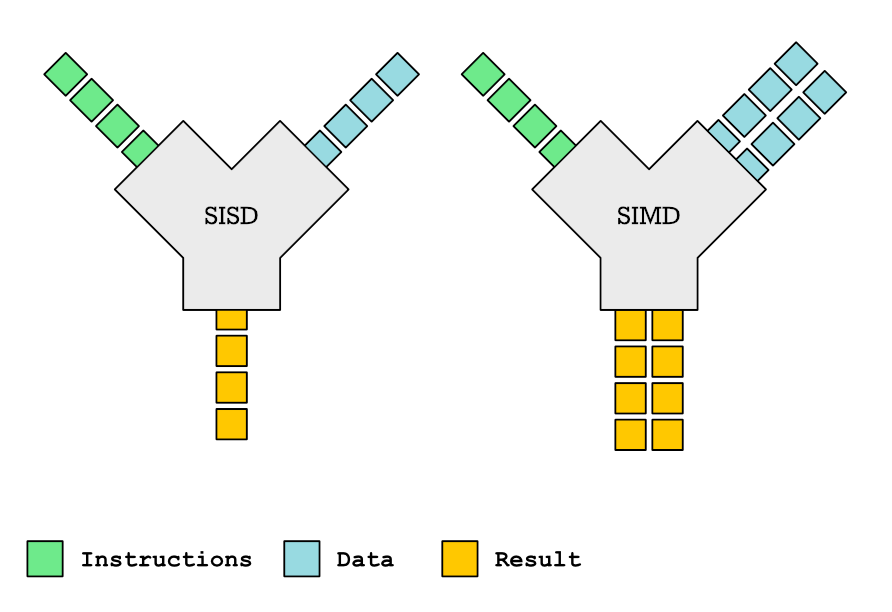
\includegraphics[width=0.5\textwidth]{images/sidd.png}
  \caption{SISD instructions\cite{bogosavljevic-2022-simd}}
\end{figure}

SIMD instructions can be found, to one degree or another, on most CPUs. Some examples of SIMD instructions are:
\href{/wiki/Intel_Corporation}{Intel}'s \href{/wiki/MMX_(instruction_set)}{MMX and iwMMXt}, \href{/wiki/Streaming_SIMD_Extensions}{SSE}, \href{/wiki/SSE2}{SSE2}, \href{/wiki/SSE3}{SSE3} \href{/wiki/SSSE3}{SSSE3} and \href{/wiki/SSE4}{SSE4.x},
\href{/wiki/Advanced_Micro_Devices}{AMD}'s \href{/wiki/3DNow!}{3DNow!}, \href{/wiki/ARC_(processor)}{ARC}'s ARC Video subsystem, \href{/wiki/SPARC}{SPARC}'s \href{/wiki/Visual_Instruction_Set}{VIS} and VIS2,
\href{/wiki/Sun_Microsystems}{Sun}'s \href{/wiki/MAJC}{MAJC}, \href{/wiki/ARM_Holdings}{ARM}'s \href{/wiki/ARM_architecture\#Advanced_SIMD_(Neon)}{Neon} technology,
\href{/wiki/MIPS_architecture}{MIPS}' \href{/wiki/MDMX}{MDMX} (MaDMaX) and \href{/wiki/MIPS-3D}{MIPS-3D}. The IBM, Sony,
Toshiba co-developed \href{/wiki/Cell_(microprocessor)}{Cell Processor}'s \href{/wiki/Synergistic_Processing_Unit}{SPU}'s instruction set is heavily SIMD based.
\href{/wiki/Philips}{Philips}, now \href{/wiki/NXP_Semiconductors}{NXP}, developed several SIMD processors named \href{/wiki/Xetal}{Xetal}. The Xetal has 320 16-bit processor elements especially designed for vision tasks.\cite{wikipedia-contributors-2025-simd}

\begin{table}[H]
  \small
  \caption{Benchmark Results for Merge Sort Iterative }
  \label{tab:mergesort-selected}
  \centering
  \begin{tabular*}{\columnwidth}{@{\extracolsep{\fill}}lccc}
    \hline
    Instruction set &  Cache size &  Data type \\
    \hline
    MMX &  64 bits &  Integer \\
    SSE &  128 bits &  Single precision Floats\\
    SSE2 &  128 bits &  Double precision Floats\\
    SSE3 &  128 bits &  Integer   \\
    SSSE3 &  128 bits &  Integer  \\
    SSE4.1 &  128 bits &  Integer \\
    \hline
  \end{tabular*}
\end{table}

\newpage

\subsection{Using Eigen}
Using SIMD for the neuron network can theoretically speed up the training process.
For in example in the activation of a neuron the dot product is computed.
Where \texttt{b} is the bias, \texttt{w} is the weights and \texttt{x} is the input vector.
The dot product is computed by multiplying the weights and inputs and adding them together.

\begin{equation}
  d (x, b) = b + \sum_{i=0}^{n} w_i \times x_i
\end{equation}

\noindent
Where this function is implemented as follows:

\begin{lstlisting}
  float Neuron::activate(const std::vector<float> &inputs)
{
    // Calculate the weighted sum of the inputs
    _lastInput = inputs;
    float weightedSum = _bias;

    // Dot product of the weights and inputs
    for (std::size_t i = 0; i < _weights.size(); i++)
    {
        weightedSum += _weights[i] * inputs[i];
    }

    // Return the result of the sigmoid function
    _lastOutput = sigmoid(weightedSum);
    return _lastOutput;
}
\end{lstlisting}
In the current implementation, the dot product is computed by explicitly looping over the weights and inputs.
This approach can be optimized by leveraging SIMD instructions.
For instance, the dot product can be calculated more efficiently using the \texttt{Eigen} library.
Alternatively, some compilers—such as \texttt{gcc}—are capable of generating SIMD instructions automatically.

\begin{lstlisting}
  float Neuron::activate(const Eigen::VectorXf &inputs)
{
    // Calculate the weighted sum of the inputs
    e_lastInput = inputs;
    e_weights = Eigen::Map<Eigen::VectorXf>(_weights.data(), _weights.size());

    // Calculate the weighted sum of the inputs
    float weightedSum = _bias + e_weights.dot(inputs);

    // Return the result of the sigmoid function
    _lastOutput = sigmoid(weightedSum);
    return _lastOutput;
}
\end{lstlisting}
Here we implemted the dot product using the \texttt{Eigen} library. The \texttt{Eigen::VectorXf} is a vector of floats.
The \texttt{Eigen::Map} function is used to map the weights vector to an \texttt{Eigen::VectorXf} vector.
Even though we map the weights vector to an \texttt{Eigen::VectorXf} vector, the performance increase we get from utilizing the SIMD instructions is noticable.
Up to 4 times faster than the previous implementation,
this makes sence because the dot product is computed for every neuron in the network with n weights and inputs, for every training pass times the number of epochs.
Hence that is why even tho we copy the weights vector to an \texttt{Eigen::VectorXf} vector, the performance increase is still noticable.

% \section{Cache}
\newpage
\section{Multi threading}
Another possible optimization is to use multi threading. Multi threading is the ability of a CPU to execute multiple processes or threads concurrently.
This can be done by using multiple cores or multiple CPUs. The CPU can switch between threads or processes to give the illusion that they are running concurrently.
This can be done by using the \texttt{std::thread} Library in C++.


\newpage
\bibliographystyle{IEEEtran}
\bibliography{IEEEabrv, references}

\end{document}